% Created 2019-11-03 Sun 19:20
% Intended LaTeX compiler: pdflatex
\documentclass[presentation]{beamer}
\usepackage[utf8]{inputenc}
\usepackage[T1]{fontenc}
\usepackage{graphicx}
\usepackage{grffile}
\usepackage{longtable}
\usepackage{wrapfig}
\usepackage{rotating}
\usepackage[normalem]{ulem}
\usepackage{amsmath}
\usepackage{textcomp}
\usepackage{amssymb}
\usepackage{capt-of}
\usepackage{hyperref}
\usepackage{minted}
\usepackage[backend=bibtex]{biblatex}
\bibliography{References}
\usepackage{amsmath, amssymb}
\usetheme{Boadilla}
\author{TODO add list of authors}
\date{November 6, 2019}
\title{Two Functional MDD's for the Price of One - Part 2}
\hypersetup{
 pdfauthor={TODO add list of authors},
 pdftitle={Two Functional MDD's for the Price of One - Part 2},
 pdfkeywords={},
 pdfsubject={},
 pdfcreator={Emacs 26.3 (Org mode 9.2.3)}, 
 pdflang={English}}
\begin{document}

\maketitle
\begin{frame}{Outline}
\tableofcontents
\end{frame}


\section{Symphony - Modeling Language for Non-Linear Optimization}
\label{sec:org5ab5078}
\begin{frame}[label={sec:org5cb1731}]{Symphony - Modeling Language for Non-Linear Optimization}
\begin{itemize}
\item Models linear and non-linear optimization problems
\item Simple declarative language
\item Support for bounded parameters and constraint programming
\item Generates performance oriented c code
\item Solver Agnostic (plug into your solver of choice)
\end{itemize}
\end{frame}
\begin{frame}[label={sec:orgf3625e4}]{SYNTAX EXAMPLES}
\end{frame}

\section{Sample Problem 1}
\label{sec:org94a0e83}
\begin{frame}[label={sec:org802260d}]{Sample Problem 1 - Velocity Problem}
\begin{center}
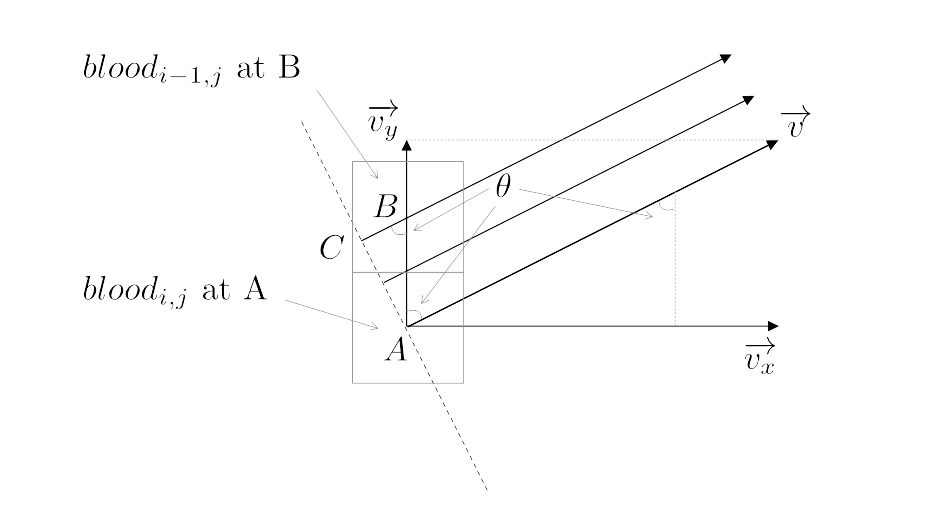
\includegraphics[width=8cm]{figs/velocity.png}
\end{center}
\begin{itemize}
\item MRI imaging problem dealing with blood flow
\item Given vector field of blood flow: can we find how long each blood cell has been there?
\item Do this by minimizing the \alert{flow} over time (hence an optimization problem!)
\end{itemize}
\end{frame}

\begin{frame}[label={sec:org03d5ffb}]{Velocity Problem - Model Derivation}
\begin{center}
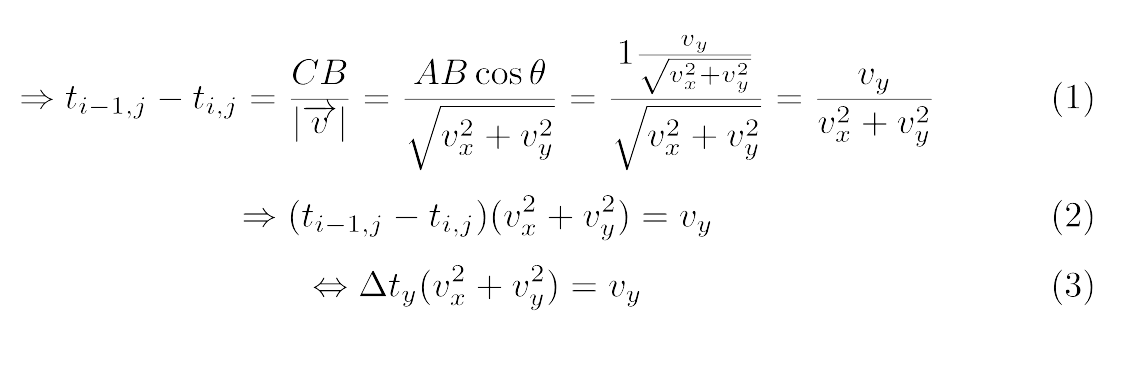
\includegraphics[width=.9\linewidth]{figs/velocityderivation.png}
\end{center}
\end{frame}
\begin{frame}[label={sec:org06e74f7}]{Velocity Problem - Optimization Model}
\begin{align*}
\textsc{min}_t &\sum_{\textsc{pixels}} (\Delta t_x (v_x^2 + v_y^2) - v_x) * v_x^2)^2  \\
               & + \sum_{\textsc{pixels}} (\Delta t_y ((v_x^2 + x_y^2) - x_y) * x_y^2)^2 \\
v_{(x,y)} \quad & \textsc{velocity in x,y direction} \\
t_{(x,y)} \quad & \textsc{time in x,y direction}
\end{align*}
\end{frame}
\section{Sample Problem 2}
\label{sec:org0fb732f}
\begin{frame}[label={sec:org0ee1152}]{Brain Problem - 1}
\begin{center}
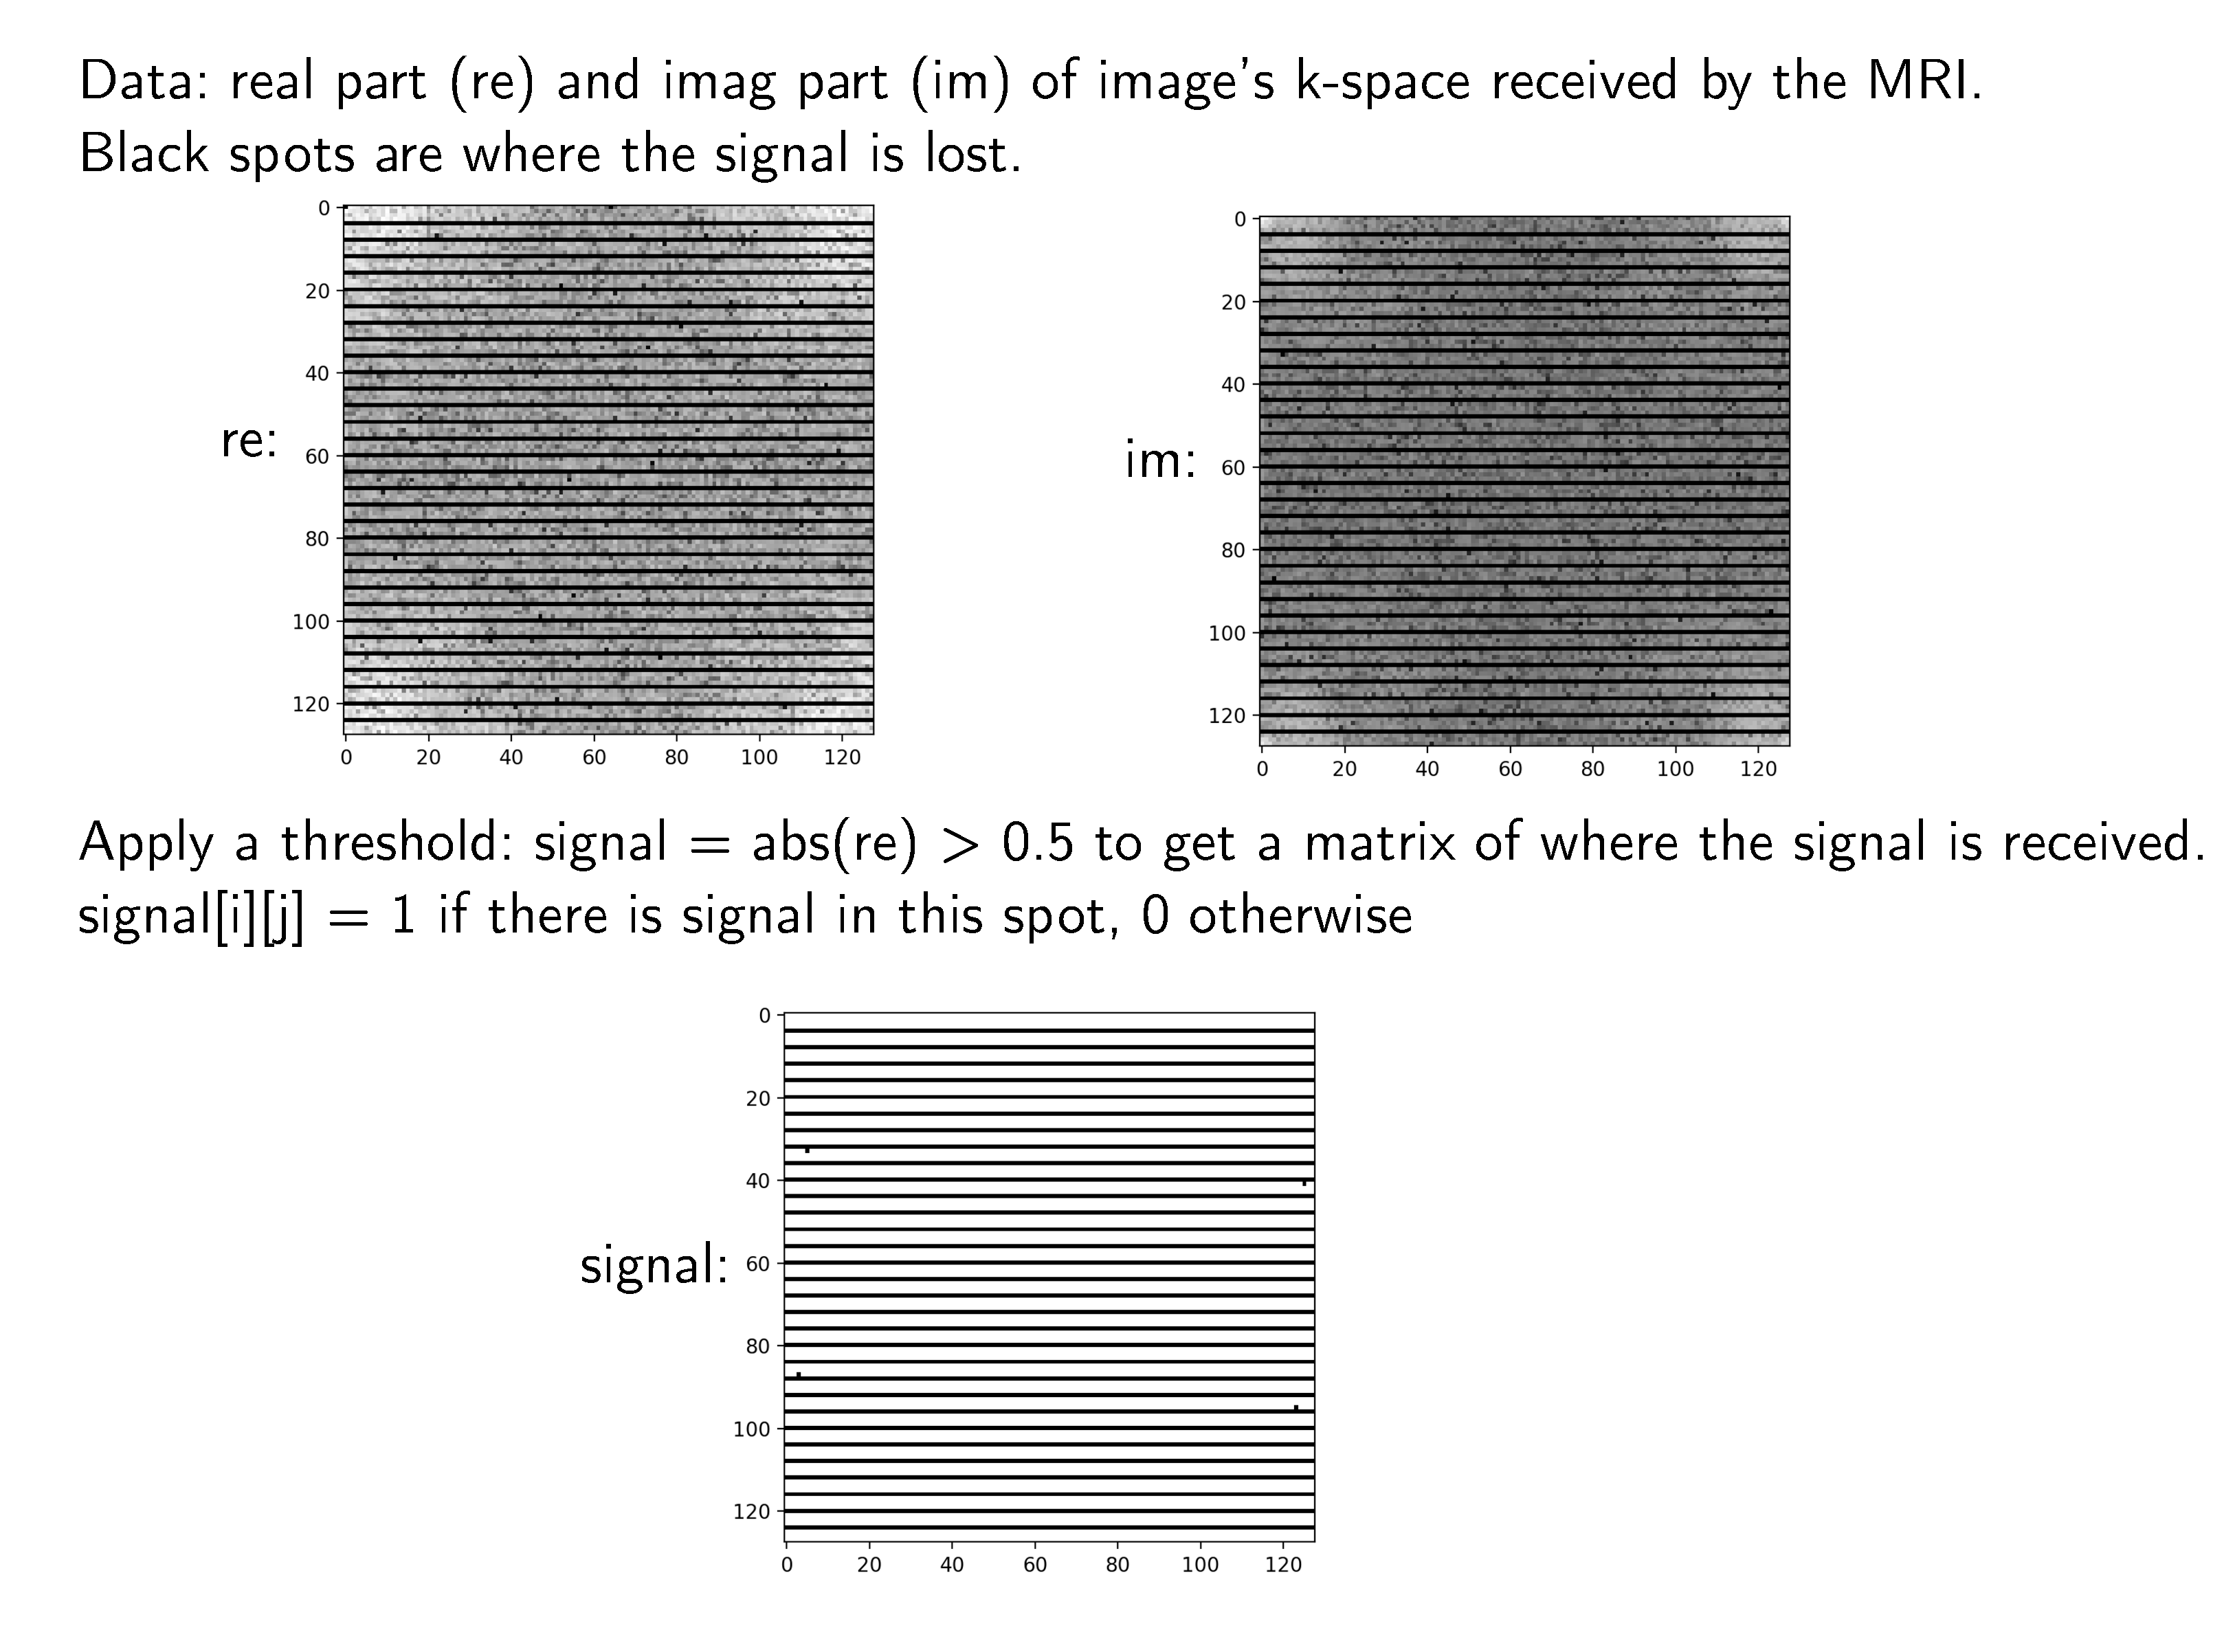
\includegraphics[width=.9\linewidth]{figs/MRIBrain1.pdf}
\end{center}
\end{frame}
\begin{frame}[label={sec:org2a77819}]{Brain Problem - 2}
\begin{center}
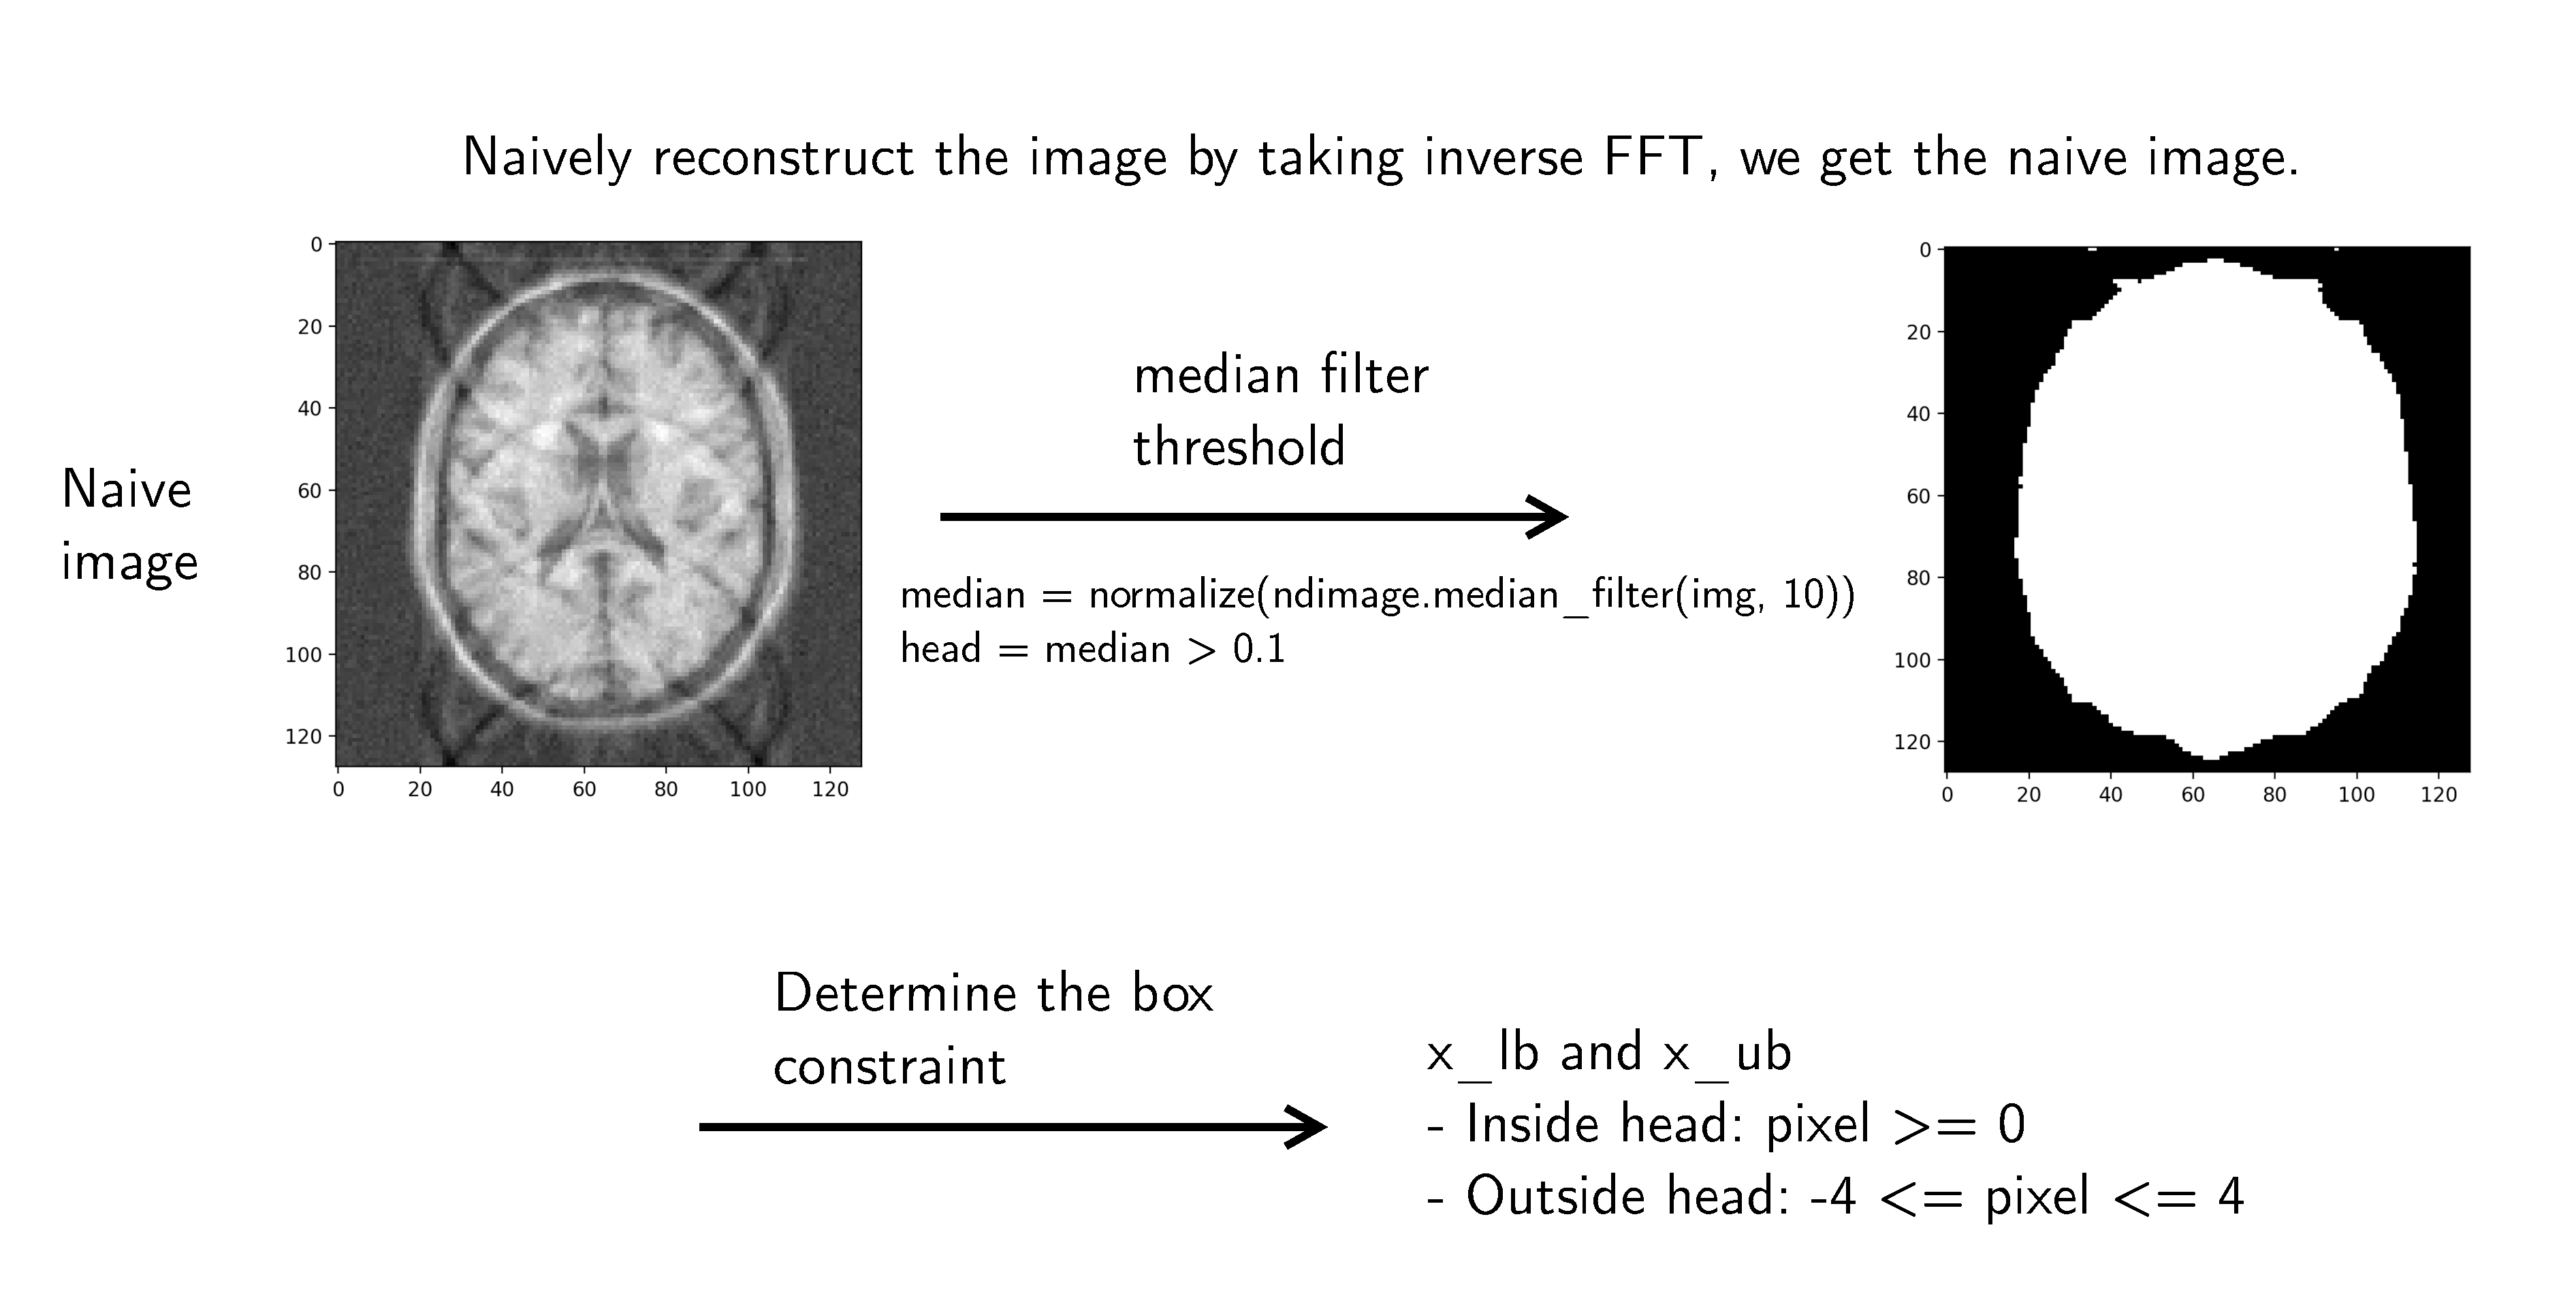
\includegraphics[width=.9\linewidth]{figs/MRIBrain2.pdf}
\end{center}
\end{frame}
\begin{frame}[label={sec:org744e067}]{Play with generating HDF5}
\end{frame}
\section{Sample Problem 3}
\label{sec:org70855ae}
\begin{frame}[label={sec:orgc46a8f9}]{(Multi-Coil MRI / Constraint Programming)}
\end{frame}
\begin{frame}[label={sec:org1b54230}]{Play with Scaling Factor}
\end{frame}
\begin{frame}[label={sec:orgff6ee47}]{Play With L2-Norm / Hubar Penalty}
\end{frame}
\section{Hashed Expression - Symphony's Backend}
\label{sec:org737f90f}
\begin{frame}[label={sec:org4426ae4}]{Hashed Expression - Symphony's Backend}
\begin{itemize}
\item Embedded Language in \alert{Haskell}
\end{itemize}
\end{frame}
\section{References}
\label{sec:org7908282}
\begin{frame}[label={sec:orga2b0704}]{References}
\printbibliography[heading=none]
\end{frame}
\end{document}